\documentclass[]{article}
\usepackage{fullpage}
\usepackage[authoryear]{natbib}
\usepackage{setspace}
    \doublespacing
\usepackage{hyperref}
\hypersetup{
    colorlinks,
    citecolor=black,
    filecolor=black,
    linkcolor=cyan,
    urlcolor=cyan
}
\usepackage{amssymb,amsmath}
\usepackage{bm}
\usepackage{dcolumn}
\usepackage{booktabs}
\usepackage{url}
\usepackage{tikz}
\usepackage{todonotes}
\usepackage[utf8]{inputenc}
\usepackage{graphicx}
\usepackage{longtable}
\usepackage{todonotes}
\usepackage{lscape}
\usepackage{float}


\title{Fiscal Rule Stretching in Europe During Financial Market Stress and Crises}

\author{Christopher Gandrud \\ \emph{City University London} \\ \emph{Hertie School of Governance}\footnote{Please contact Christopher Gandrud
(\href{mailto:christopher.gandrud@city.ac.uk}{\nolinkurl{christopher.gandrud@city.ac.uk}}) or Mark Hallerberg (\href{mailto:hallerberg@hertie-school.org}{\nolinkurl{hallerberg@hertie-school.org}}). Full data and replication material can be found at: \url{https://github.com/christophergandrud/eurostat_revisions}.}
\and
Mark Hallerberg \\ \emph{Hertie School of Governance}}

\begin{document}

\maketitle

\begin{center}
    \textbf{Very Early Working Draft for\\ Texas A \& M University: Fiscal Policy in Europe Workshop (10-11 December 2015) \\
    Comments and suggestions very welcome.}
\end{center}

\begin{abstract}
    Elected governments have incentives to stretch accounting rules by classifying loss-making and/or indebted endeavors, such as public industries and pension schemes, as off of the public balance sheet. Doing so improves the appearance of the incumbent government to cost-conscious voters. We expect rule stretching to be especially prevalent during periods of financial market stress and crises given the typically high expense of responding to these events. In addition, types of policy options available to assist troubled financial institutions, such as bad banks and bank nationalizations, are often hard to classify as being inside or outside of the government sector, thus making it more likely that governments will tend to stretch how they are classified. To test these proposition, we examine revisions to government debt and deficit figures made by the European statistical agency--Eurostat. These revisions frequently occur because this politically independent agency re-classifies member state created organizations as being within the government sector, when a national government had originally classified them as outside. We find that debt figures are more likely to be revised upwards for years close to national elections, especially when these are endogenous elections. Such election effects are strengthened further by financial market stress. Our research underlines the importance of having a vigilant and politically independent government statistical agency during periods of financial market stress to ensure reliable government finance statistics.
\end{abstract}

\section{Introduction}

This paper examines why governments manipulate their publicly reported data on debt and deficits. This research question affects other literatures in political science in interesting ways. One strand examines the relationship between the reporting of data and the quality of governance (e.g., Hollyer, Rosendorff, and Vreeland 2014).  \cite{Alt2014} explore the relationship among the transparency of fiscal data, elections and pressure from the European Union. Another strand focuses on the economic vote, and it finds that voters generally do not pay attention to revised figures (see Kayser and Peress 2015).

While their focus is on the role of the media in reporting such figures, our paper builds on the insights in Kayser and Peress and on Alt, Lassen, and Wehner’s work on elections and transparency to explore the implications of their argument for government action. If voters care most about reported, rather than actual, figures then governments have an incentive to manipulate them before elections. One would expect greater manipulation in ways that make the government look better as elections approach. We can measure these activities by looking at revisions of budget figures, and particularly debt. We also explore three alternative hypotheses. The first centers on the role of international institutions. Governments may report figures in ways to please an international actor, which in turn can damage the standing of the government in the eyes of its voters. The second considers institutional arguments about who does the numbers. In some countries, the government does the reporting, while in others an independent body plays this role. The final alternative focuses on “shocks” to the economy, which in turn affect government statistics. Countries with more shocks may engage in more revisions, with the bias depending upon the nature of the shocks (positive or negative). Of course, these three arguments may be related in theoretically interesting ways. For example, a country experiencing a positive shock may be more likely to call an election in countries where elections are endogenous.

Our dataset is composed only of European Union member states. This is useful for several reasons. They face one international organisation that has two sets of rules on economic matters for its members that are often closely related, namely those rules for Member States inside the eurozone and those outside. The face one accounting regime and they have one body, Eurostat, that enforces it. This means that differences across countries are less likely to be because of different accounting standards. They are all parliamentary or semi-presidential systems where parliamentary elections are crucial for the formation of governments.

We find that...

\section{Political budget cycles and fiscal gimmicks}

The revision of government-reported statistics is of interest for several reasons.

The reporting of statistics, or the lack of it,  may tell one about the overall governance of a given country. \cite{Hollyer2014} argue that the lack of reporting is not random. They collect the availability of data for 125 over a thirty-year period and they use a Bayesian Item Response  (IRT) model to create a transparency index.  They use this data to predict the quality of governance in autocracies. In other work, they anticipate that this type of transparency affects government accountability as well as collective action (\cite{Hollyer2016}). \footnote{\cite{Jervin:2013} tells a similar story for African countries. The quality of data is generally good when governments have state capacity to provide them. When those governments get in trouble, however, so that their capacity declines the quality of the data also drops.}

While \cite{Hollyer2014} consider how voters might react when they get data, there is a separate literature that focuses on how voters react, and in particular whether signals they receive from economic data about the competence of the government in managing economic policy. One debate considers whether voters or prospective or retrospective. On the latter, the assumption is that voters observe outcomes, and they decide whether to support the incumbent government. There is a growing literature on “real-time fiscal policy.” Kayser and Peress (2015) find that...

We build on this insight for the first explanation that we examine. Building on \cite{Nordhaus1975}, one would anticipate that there are opportunistic business cycles where governments manipulate macro-economic tools at their disposal in an effort to make the economy look better before an election. Clark (2003) finds the the tools one uses depends upon the logic of the Mundell-Fleming model: if one assumes that capital is mobile, governments use monetary policy when the exchange rate is flexible and fiscal policy when the exchange rate is fixed. Both Nordhaus and Clark, however, focus on actual economic output from the use of these instruments. We are interested in the perceived figures prior to an election. There is  a possible spin-off on the Clark argument. One can expect that extra spending in EU member states with flexible exchange rates has no macro-economic payoffs, while it does have payoffs in countries with fixed exchange rates, which will mostly be those in the eurozone. \footnote{Exceptions would be those countries that fix their exchange rate to the euro or that have very narrow bands. Some central and East European Countries, for example, had currency boards that maintained a de facto fix. Denmark has chosen not to join the eurozone, but it maintains a tight fix between its kronor and the euro.}

There is evidence that countries intentionally distort statistics so that they receive some sort of payoff from an international organisation. For example, \cite{Kerneretal2014} find that some African countries kept their per capita incomes below the  eligibility threshold for World
Bank’s International Development Association (IDA).  This is a clear case where governments change their official statistics in response to an expectation from an international organization.

Reported outcomes in terms of economic and fiscal data have a real impact on policy especially in European Union countries. GDP figures affect what type of co-financing governments receive from the European Union for a range of activities, such as environmental protection, guarantees for loans that Small and Medium-sized Enterprises (SMEs) take, and the construction of roads. \footnote{The amounts can be substantial as a percentage of total funding for a given project, up to 85 percent of the cost of the project in regions judged to be “”, which are those with a per capita income below 75 percent of the European Union average.} Under the Stability and Growth Pact, all Member States are expected to have budget balances no worse than 3 percent of GDP and debt burden no greater than 60 percent of GDP. The European Commission decides each year whether a member state has an “excessive deficit,” with those earning this distinction under the Commission subject to an “excessive deficit procedure.” Member states must propose corrective methods. The subset that are also eurozone members face potential penalties, such as fines. Member states that do not adjust their performance also could lose their access to structural and cohesion funds, which are the largest part of the European Union budget.

One could ask whether countries that have clear biases concerning future performance have similar biases concerning current performance. A literature on forecasting considers why there are biases in forecasting numbers. Some governments seem to be eternal optimists; they report figures that that always appear to be better than turn out to be. Others are chronic pessimists, and they have positive “surprises.” Looking at European Union member states, work from the early years of the euro finds that (\cite{HallerbergStrauch2002}). In more recent work, Hallerberg, et al. (2009) find that European Union member states that fit most closely a “fiscal contracts” approach to budgeting have more conservative forecasts than member states that fit better a “delegation to a strong finance minister” approach.

This discussion leads us to an institutional argument to explore. \todo{one could explore these intra-governmental differences as well if space/time/interest. The predictions, however, are not so clean. I can imagine that if you have fiscal contracts—say you are the Netherlands—you might fudge numbers so the you more or less comply with internal targets. If it turns out later you missed a bit, you probably won’t bring down the government. At the same time, precisely because of there is a temptation to do this you might have especially competent staff do the numbers.}

\cite{DeCastro2013} \cite{Alt2014}

\section{Cost-shifting during financial crises}

\cite{GandrudHallerberg2016}

\section{Hypotheses}

\begin{quote}
    $H_{1}$: Debt revisions will be smaller for years further from national government elections.
\end{quote}

\begin{quote}
    $H_{2}$: Debt revisions will be greater for years when there are endogenous elections.
\end{quote}

\begin{quote}
    $H_{3}$: The effects predicted by $H_{1}$ and $H_{2}$ will be stronger when a country also has high credit provision stress.
\end{quote}

\section{Empirical tests}

To test our hypotheses, we ran a series of linear regressions with cumulative debt and deficit revisions made by Eurostat as the dependent variable and a number of relevant political and economic indicators on the right-hand side.

\subsection{Eurostat revisions}

To test these hypotheses we gathered all of the revisions that Eurostat made to EU member debt and deficit figures from 2003 through 2013.\footnote{PDF files with the figures were downloaded from \url{http://ec.europa.eu/eurostat/news/news-releases}. Accessed March 2015.} Eurostat publishes revisions bi-annually--typically once at the end of April and again again in late October. These revisions cover government finance statistics released within the previous four years. As such, the unit of analysis in the following regressions is biannual revision point for each fiscal year. For every year that government statistics are revised, there are up to seven revision points.\footnote{The first revisions occur October of the initial reporting year.}

We created a variable of \emph{cumulative revisions for debts and deficits} over these four year periods and used them as our dependent variables. For debt revisions, it ranged from -1.1 and 12.7 percent of GDP. For deficit revisions it ranged from -4.5 and 1.1 percent of GDP. It is important to note that all of these revisions were not due to revisions in the denominator, i.e. GDP. Eurostat reports these types of changes separately. As \cite{DeCastro2013} found for similar Eurostat data in shorter pre-financial crisis sample, there is a clear tendency for debt statistics to be revised upward and deficit statistics downward, indicating that policies are more expensive than initially reported.

\subsection{Right-hand variables}

To test whether governments are more likely to stretch the rules closer to elections, we use Gandrud's \citeyearpar{gandrudYrcurnt} \emph{years to election} variable. The election year is recorded as zero. Not only do we expect that governments are more likely to use rule stretching as elections approach, but that rule stretching should be more prevalent when governments are not able to choose the when the election occurs so as to present themselves in the best fiscal light to voters. As such, we also include a dummy variable that is one for \emph{required elections} (e.g. non-endogenous elections) and zero for all other years. The variable is from \cite{Brender2008}. It was updated and corrected by Hallerberg and Wehner. We expect that that revisions will be greater for years when there is a non-endogenous election.

To examine how responding to financial market stress may exacerbate governments' fiscal accounting rule stretching behavior, we included Gandrud and Hallerberg's \citeyearpar{finstress_paper} continuous ``FinStress'' measure of real-time perceptions of financial market stress. This measure is created by analyzing monthly content from Economist Intelligence Unit texts on banking and financial markets using a statistical method called kernel principal component analysis. Unlike previous post-hoc dichotomous measures of financial crisis \citep[e.g. measures compiled by][]{Laeven2012,ReinhartRog2010}, the authors argue this measure captures what we are most interested in when trying to understand policy choices: what stress policy-makers perceived and so responded to at the time. It also does not rely on ad hoc methods of determining when a crisis ended, but instead charts its perceived intensity over time. To make this measure comparable with our other variables, we found yearly averages. FinStress is able to vary between zero and one, with higher values indicating more perceived financial market stress. In the sample it varies between 0.12 and 0.76.

Because hypothesize that the effect of election timing on rule-stretching will increase at higher levels of financial market stress, we will focus on interacting FinStress with the election timing and non-endogenous elections variables.

As Eurostat has more time to examine member state government policies, e.g. how separate they are in practice from the government sector, we would expect on average that the cumulative revisions will grow over the course of the four year period during which they are revised. So we also include a variable counting the years since the original year that the revised figure is from on the right-hand side.

We also examined whether the level of government debts and deficits effects the propensity of rule stretching and therefore revisions by Eurostat. We gather general government deficits as a percentage of GDP from Eurostat.\footnote{Available at: \url{http://ec.europa.eu/eurostat/}. Accessed December 2015.} For debts, we use information reported by the World Bank's Development Indicators.\footnote{Available at: \url{http://data.worldbank.org/data-catalog/world-development-indicators}. Accessed December 2015.} Both sets of numbers were updated by 2015.

\subsection{Results}

Tables \ref{debt_results} and \ref{deficit_results} show our results from linear regressions with cumulative debt and deficit revisions as the dependent variables, respectively. All models include country fixed effects.

\subsection{Debt Revisions}

We can see in Table \ref{debt_results} model 3 that years from an election is estimated to have a negative effect on debt revisions in models where it is not interacted with FinStress. Government debt figures tend to be revised less for years further away from the next election. Or stated another way, debt revisions are larger for years closer to elections. This finding is similar in direction and magnitude to what \cite{DeCastro2013} previously uncovered with similar data over a shorter time-span. New findings can be seen in subsequent models of Table \ref{debt_results}. In model 4 we can see that debt revisions were larger in endogenous election years, where a government called an election when they were not required to. Conversely, non-endogenous election years see no difference in debt revisions compared to non-election years. Looking at the interactive models (7-9), their findings are in line with our third hypothesis that the two election effects increase for years that also have higher credit market stress as measured by the FinStress variable.

To understand the direction and magnitude of these interactive effects, figures \ref{me_finstress_elect} and \ref{me_finstress_endog_elect} show marginal effects of the election variables at various levels of credit market stress. At high levels of FinStress, e.g. above 0.55,\footnote{\cite{finstress_paper} find that countries classified by \cite{Laeven2012} as being in banking crises tend to have FinStress scores above 0.55, especially in developed economies such as those found in the EU.} the marginal effect of being one more year removed from an election on debt revisions is about -0.2 percentage points of GDP. Figure \ref{me_finstress_endog_elect} shows that having an endogenous election during a similar high stress period increases debt revisions by about 2 percentage points of GDP.

To get a sense of how these average effects may play out in each country, we predicted the debt revisions by the fourth revision year for 27 EU member states.\footnote{We did not include the newest member--Croatia--as its figures have been subject to Eurostat oversight for relatively few years.} Using estimates shown in model 8 of Table \ref{debt_results}, we predicted revisions for non-election years, endogenous election years, and non-endogenous election years at observed country minimum and maximum FinStress values. The predictions are shown in Figure \ref{country_predict_debt_required}. Please note that while we used observed country FinStress ranges these plots make frequent out of sample predictions as most countries did not have endogenous and non-endogenous elections at these levels of stress. Basic country effects correspond to our priors, namely Greece has very large revisions regardless of election year and type. Typically, when countries are fitted to have endogenous elections at high stress levels, e.g. Belgium, Denmark, Latvia, Ireland, Spain, and so on, we predict that their debt figures will be revised by about 3.25 percentage points of GDP.



\subsection{Deficit Revisions}

We also examined if election type and election timing affected the need for revisions to governments' deficit figures (Table \ref{deficit_results}). First, it is interesting to note that while higher debt levels did not appear to be related to debt figures that required more revisions, higher deficit levels are associated with higher deficit revisions. Perhaps this is related to the primary importance of the 3 percent deficit target by Stability and Growth Pact monitors, until the Eurozone debt crisis.\footnote{Remember that the sample used in our regressions goes through 2011, only one year after the real start of the debt crisis.}

Onto the electoral and financial market stress variables. There does not appear to be an interactive relationship between financial market stress and years to election on deficit revisions. This could be because responses to financial market stress--bank nationalizations, guarantees, and so on--predominantly impact government debts rather than deficits. There does appear to be a statistically significant relationship between non-endogenous elections and FinStress that is similar to the interaction between endogenous elections and stress in the debt revisions models (see \ref{me_finstress_non_endog_deficit} for the marginal effects). More work is needed to understand this finding.

\begin{landscape}
    
% Table created by stargazer v.5.2 by Marek Hlavac, Harvard University. E-mail: hlavac at fas.harvard.edu
% Date and time: Fri, Feb 12, 2016 - 14:39:59
\begin{table}[!htbp] \centering 
  \caption{Linear Regression Estimation of \textbf{Debt} Revisions} 
  \label{debt_results} 
\tiny 
\begin{tabular}{@{\extracolsep{5pt}}lccccccccccc} 
\\[-1.8ex]\hline 
\hline \\[-1.8ex] 
 & \multicolumn{11}{c}{\textit{Dependent variable:}} \\ 
\cline{2-12} 
\\[-1.8ex] & \multicolumn{11}{c}{Cumulative Debt Revisions} \\ 
\\[-1.8ex] & (1) & (2) & (3) & (4) & (5) & (6) & (7) & (8) & (9) & (10) & (11)\\ 
\hline \\[-1.8ex] 
 Cum. Revisions (lag) & 0.628$^{***}$ & 0.757$^{***}$ & 0.626$^{***}$ & 0.731$^{***}$ & 0.554$^{***}$ & 0.536$^{***}$ & 0.641$^{***}$ & 0.640$^{***}$ & 0.634$^{***}$ & 0.681$^{***}$ & 0.634$^{***}$ \\ 
  & (0.021) & (0.021) & (0.021) & (0.022) & (0.026) & (0.026) & (0.021) & (0.021) & (0.022) & (0.025) & (0.022) \\ 
  & & & & & & & & & & & \\ 
 Election Timing & 0.047$^{*}$ &  & $-$0.031 &  &  &  &  &  & $-$0.064 &  & $-$0.028 \\ 
  & (0.027) &  & (0.047) &  &  &  &  &  & (0.049) &  & (0.040) \\ 
  & & & & & & & & & & & \\ 
 Unscheduled Elect. &  & 0.229$^{*}$ &  & $-$0.560$^{**}$ &  &  &  &  &  & $-$0.576$^{**}$ &  \\ 
  &  & (0.132) &  & (0.235) &  &  &  &  &  & (0.248) &  \\ 
  & & & & & & & & & & & \\ 
 Scheduled Elect. &  & $-$0.001 &  & $-$0.057 &  &  &  &  &  & $-$0.157 &  \\ 
  &  & (0.073) &  & (0.128) &  &  &  &  &  & (0.150) &  \\ 
  & & & & & & & & & & & \\ 
 Financial Stress & 0.039 & 0.191 & $-$1.082$^{*}$ & $-$0.049 &  &  &  &  & $-$1.380$^{**}$ & $-$0.001 & 0.075 \\ 
  & (0.327) & (0.257) & (0.643) & (0.278) &  &  &  &  & (0.651) & (0.331) & (0.343) \\ 
  & & & & & & & & & & & \\ 
 Gen. Gov. Deficit &  &  &  &  & $-$0.004 & 0.010 &  &  &  &  &  \\ 
  &  &  &  &  & (0.011) & (0.011) &  &  &  &  &  \\ 
  & & & & & & & & & & & \\ 
 Cent. Gov. Debt &  &  &  &  & 0.004$^{*}$ & 0.004$^{*}$ &  &  &  &  &  \\ 
  &  &  &  &  & (0.002) & (0.002) &  &  &  &  &  \\ 
  & & & & & & & & & & & \\ 
 Euro Member &  &  &  &  & 0.233 & $-$0.479$^{*}$ & $-$0.006 & $-$0.066 &  &  &  \\ 
  &  &  &  &  & (0.183) & (0.272) & (0.194) & (0.201) &  &  &  \\ 
  & & & & & & & & & & & \\ 
 EDP &  &  &  &  &  &  & 0.163$^{**}$ & 0.041 & 0.175$^{**}$ & 0.083 & $-$0.145 \\ 
  &  &  &  &  &  &  & (0.080) & (0.131) & (0.082) & (0.081) & (0.155) \\ 
  & & & & & & & & & & & \\ 
 Elect. Timing*Fin. Stress &  &  & 0.506$^{**}$ &  &  &  &  &  & 0.658$^{***}$ &  &  \\ 
  &  &  & (0.250) &  &  &  &  &  & (0.252) &  &  \\ 
  & & & & & & & & & & & \\ 
 Unscheduled.Elect*Fin. Stress &  &  &  & 5.818$^{***}$ &  &  &  &  &  & 6.493$^{***}$ &  \\ 
  &  &  &  & (1.443) &  &  &  &  &  & (1.524) &  \\ 
  & & & & & & & & & & & \\ 
 Scheduled.Elect*Fin. Stress &  &  &  & 0.384 &  &  &  &  &  & 0.980 &  \\ 
  &  &  &  & (0.731) &  &  &  &  &  & (0.815) &  \\ 
  & & & & & & & & & & & \\ 
 Cent. Gov. Debt*Euro &  &  &  &  &  & 0.011$^{***}$ &  &  &  &  &  \\ 
  &  &  &  &  &  & (0.003) &  &  &  &  &  \\ 
  & & & & & & & & & & & \\ 
 EDP*Euro &  &  &  &  &  &  &  & 0.191 &  &  &  \\ 
  &  &  &  &  &  &  &  & (0.162) &  &  &  \\ 
  & & & & & & & & & & & \\ 
 Elect. Timing*EDP &  &  &  &  &  &  &  &  &  &  & 0.137$^{**}$ \\ 
  &  &  &  &  &  &  &  &  &  &  & (0.057) \\ 
  & & & & & & & & & & & \\ 
 Constant & 0.648$^{***}$ & 0.361$^{**}$ & 0.831$^{***}$ & 0.353$^{**}$ & 0.251 & 0.316 & 0.658$^{**}$ & 0.688$^{***}$ & 0.807$^{***}$ & 0.343$^{**}$ & 0.752$^{***}$ \\ 
  & (0.188) & (0.151) & (0.208) & (0.152) & (0.309) & (0.308) & (0.255) & (0.257) & (0.209) & (0.160) & (0.203) \\ 
  & & & & & & & & & & & \\ 
\hline \\[-1.8ex] 
Country FE? & Yes & Yes & Yes & Yes & Yes & Yes & Yes & Yes & Yes &  &  \\ 
Observations & 1,494 & 1,189 & 1,494 & 1,189 & 1,230 & 1,230 & 1,371 & 1,371 & 1,345 & 1,047 & 1,345 \\ 
R$^{2}$ & 0.546 & 0.655 & 0.547 & 0.660 & 0.397 & 0.403 & 0.546 & 0.546 & 0.548 & 0.636 & 0.548 \\ 
Adjusted R$^{2}$ & 0.537 & 0.646 & 0.538 & 0.651 & 0.384 & 0.390 & 0.536 & 0.536 & 0.538 & 0.625 & 0.537 \\ 
\hline 
\hline \\[-1.8ex] 
\textit{Note:}  & \multicolumn{11}{r}{$^{*}$p$<$0.1; $^{**}$p$<$0.05; $^{***}$p$<$0.01} \\ 
\end{tabular} 
\end{table} 

\end{landscape}

\begin{landscape}
    
% Table created by stargazer v.5.2 by Marek Hlavac, Harvard University. E-mail: hlavac at fas.harvard.edu
% Date and time: Thu, Oct 27, 2016 - 13:37:08
\begin{table}[!htbp] \centering 
  \caption{Linear Regression Estimation of Deficit Revisions (Full Sample)} 
  \label{deficit_results} 
\tiny 
\begin{tabular}{@{\extracolsep{5pt}}lcccccccccc} 
\\[-1.8ex]\hline 
\hline \\[-1.8ex] 
 & \multicolumn{10}{c}{\textit{Dependent variable:}} \\ 
\cline{2-11} 
\\[-1.8ex] & \multicolumn{10}{c}{Cumulative Deficit Revisions} \\ 
\\[-1.8ex] & (1) & (2) & (3) & (4) & (5) & (6) & (7) & (8) & (9) & (10)\\ 
\hline \\[-1.8ex] 
 Revised Gen. Gov. Deficit & 0.053$^{***}$ & 0.042$^{*}$ & 0.042$^{*}$ & 0.048$^{***}$ & 0.049$^{***}$ & 0.049$^{***}$ & 0.038$^{**}$ & 0.050$^{***}$ & 0.033$^{**}$ & 0.098$^{**}$ \\ 
  & (0.013) & (0.020) & (0.020) & (0.013) & (0.013) & (0.013) & (0.013) & (0.014) & (0.011) & (0.030) \\ 
  & & & & & & & & & & \\ 
 Euro Member & $-$0.190 & $-$0.180 & $-$0.180 & $-$0.183 & $-$0.192 & $-$0.205 & $-$0.145 & $-$0.179 & $-$0.329 & $-$0.353 \\ 
  & (0.197) & (0.193) & (0.193) & (0.182) & (0.181) & (0.182) & (0.188) & (0.190) & (0.262) & (0.212) \\ 
  & & & & & & & & & & \\ 
 EDP & 0.340$^{**}$ &  &  &  &  &  &  &  &  & 0.346$^{**}$ \\ 
  & (0.104) &  &  &  &  &  &  &  &  & (0.112) \\ 
  & & & & & & & & & & \\ 
 Election Timing &  &  &  & $-$0.014 &  &  &  & $-$0.038 &  &  \\ 
  &  &  &  & (0.027) &  &  &  & (0.124) &  &  \\ 
  & & & & & & & & & & \\ 
 Unscheduled Elect. &  &  &  &  & $-$0.163 & 0.663 &  &  &  & 0.518 \\ 
  &  &  &  &  & (0.153) & (0.640) &  &  &  & (0.661) \\ 
  & & & & & & & & & & \\ 
 Scheduled Elect. &  &  &  &  & 0.115 & $-$0.197 &  &  &  & $-$0.349 \\ 
  &  &  &  &  & (0.090) & (0.369) &  &  &  & (0.427) \\ 
  & & & & & & & & & & \\ 
 Financial Stress &  &  &  & 0.008 & 0.009$^{*}$ & 0.009 &  & 0.007 &  & 0.005 \\ 
  &  &  &  & (0.004) & (0.004) & (0.005) &  & (0.008) &  & (0.006) \\ 
  & & & & & & & & & & \\ 
 Fiscal Transparency &  &  &  &  &  &  & $-$0.001 & $-$0.0003 &  &  \\ 
  &  &  &  &  &  &  & (0.003) & (0.003) &  &  \\ 
  & & & & & & & & & & \\ 
 GDP Growth &  &  &  &  &  &  & $-$0.008 & $-$0.003 &  & $-$0.004 \\ 
  &  &  &  &  &  &  & (0.010) & (0.010) &  & (0.012) \\ 
  & & & & & & & & & & \\ 
 Contracts &  &  &  &  &  &  &  &  & $-$0.669 &  \\ 
  &  &  &  &  &  &  &  &  & (1.999) &  \\ 
  & & & & & & & & & & \\ 
 Debt * Euro &  & $-$0.013 & $-$0.013 &  &  &  &  &  &  & $-$0.042 \\ 
  &  & (0.024) & (0.024) &  &  &  &  &  &  & (0.029) \\ 
  & & & & & & & & & & \\ 
 Elect. Timing * Fin. Stress &  &  &  &  &  & $-$0.017 &  &  &  & $-$0.016 \\ 
  &  &  &  &  &  & (0.013) &  &  &  & (0.013) \\ 
  & & & & & & & & & & \\ 
 Unscheduled Elect. * Fin. Stress &  &  &  &  &  & 0.007 &  &  &  & 0.011 \\ 
  &  &  &  &  &  & (0.008) &  &  &  & (0.009) \\ 
  & & & & & & & & & & \\ 
 Scheduled Elect. * Fin. Stress &  &  &  &  &  &  &  & 0.001 &  &  \\ 
  &  &  &  &  &  &  &  & (0.003) &  &  \\ 
  & & & & & & & & & & \\ 
 Constant & $-$0.322 & $-$0.303 & $-$0.303 & $-$0.654$^{*}$ & $-$0.696$^{*}$ & $-$0.704$^{*}$ & $-$0.265 & $-$0.551 & 0.464 & $-$0.428 \\ 
  & (0.267) & (0.259) & (0.259) & (0.314) & (0.310) & (0.324) & (0.273) & (0.457) & (1.839) & (0.381) \\ 
  & & & & & & & & & & \\ 
\hline \\[-1.8ex] 
Country FE? & Yes & Yes & Yes & Yes & Yes & Yes & Yes & Yes & Yes & Yes \\ 
Observations & 413 & 460 & 460 & 460 & 460 & 460 & 460 & 460 & 423 & 413 \\ 
R$^{2}$ & 0.286 & 0.267 & 0.267 & 0.274 & 0.279 & 0.283 & 0.268 & 0.274 & 0.265 & 0.306 \\ 
Adjusted R$^{2}$ & 0.232 & 0.216 & 0.216 & 0.221 & 0.225 & 0.226 & 0.215 & 0.216 & 0.215 & 0.240 \\ 
\hline 
\hline \\[-1.8ex] 
\textit{Note:}  & \multicolumn{10}{r}{$^{*}$p$<$0.05; $^{**}$p$<$0.01; $^{***}$p$<$0.001} \\ 
\end{tabular} 
\end{table} 

\end{landscape}


\begin{figure}
    \caption{Marginal Effect of Election Timing (years to election) at Various Levels of Financial Market Stress on \textbf{Debt} Revisions}
    \label{me_finstress_elect}

    \begin{center}
        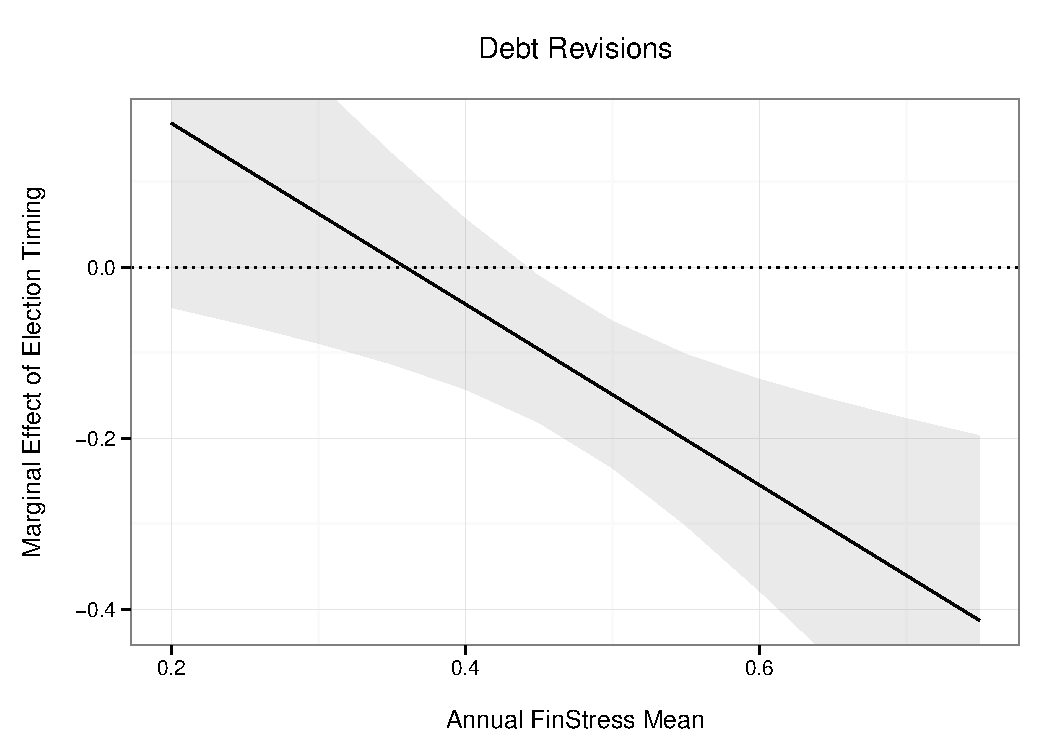
\includegraphics[scale=0.4]{figures/finstress_elect_me.pdf}
    \end{center}

	{\scriptsize{Shaded area represents 95\% confidence interval.}}

\end{figure}

\begin{figure}
    \caption{Marginal Effect of an Endogenous Election at Various Levels of Financial Market Stress on \textbf{Debt} Revisions}
    \label{me_finstress_endog_elect}

    \begin{center}
        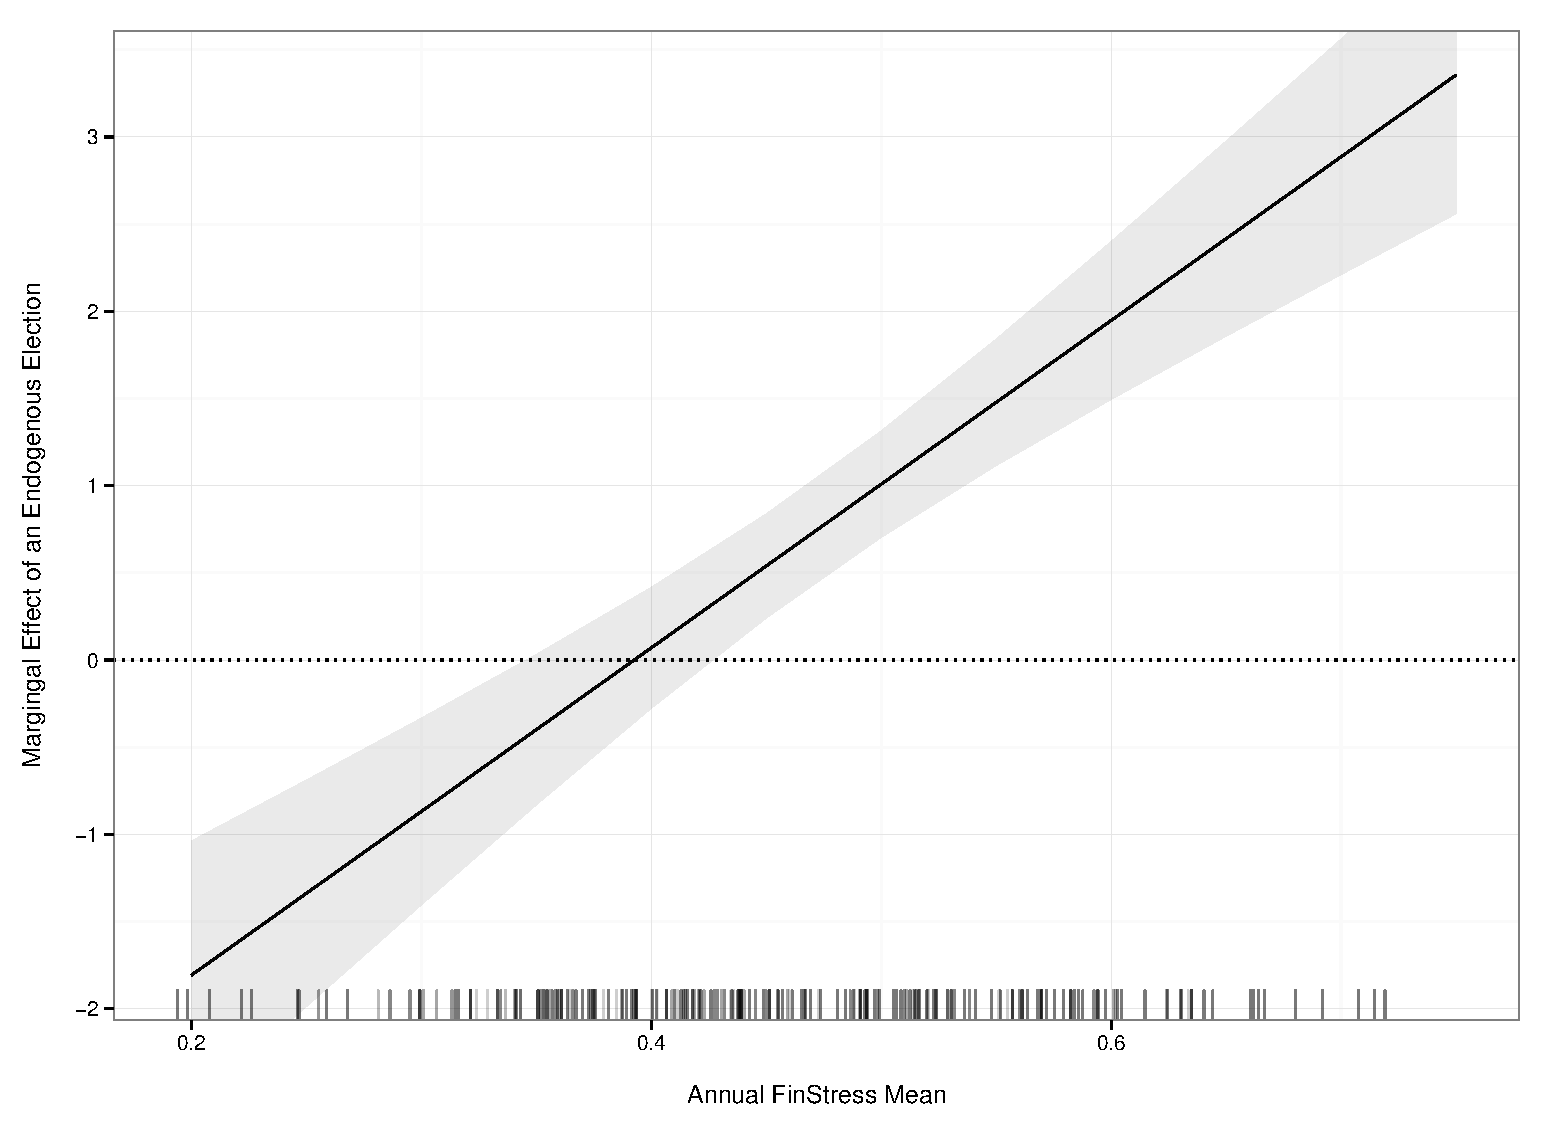
\includegraphics[scale=0.4]{figures/finstress_endog_elect_me.pdf}
    \end{center}

	{\scriptsize{Shaded area represents 95\% confidence interval.}}

\end{figure}

\begin{figure}
	\caption{Predicted \textbf{Debt} Revisions in Four Years After Publication for Years with Different Election Types/Non-election Years}
    \label{country_predict_debt_required}
    \begin{center}
    	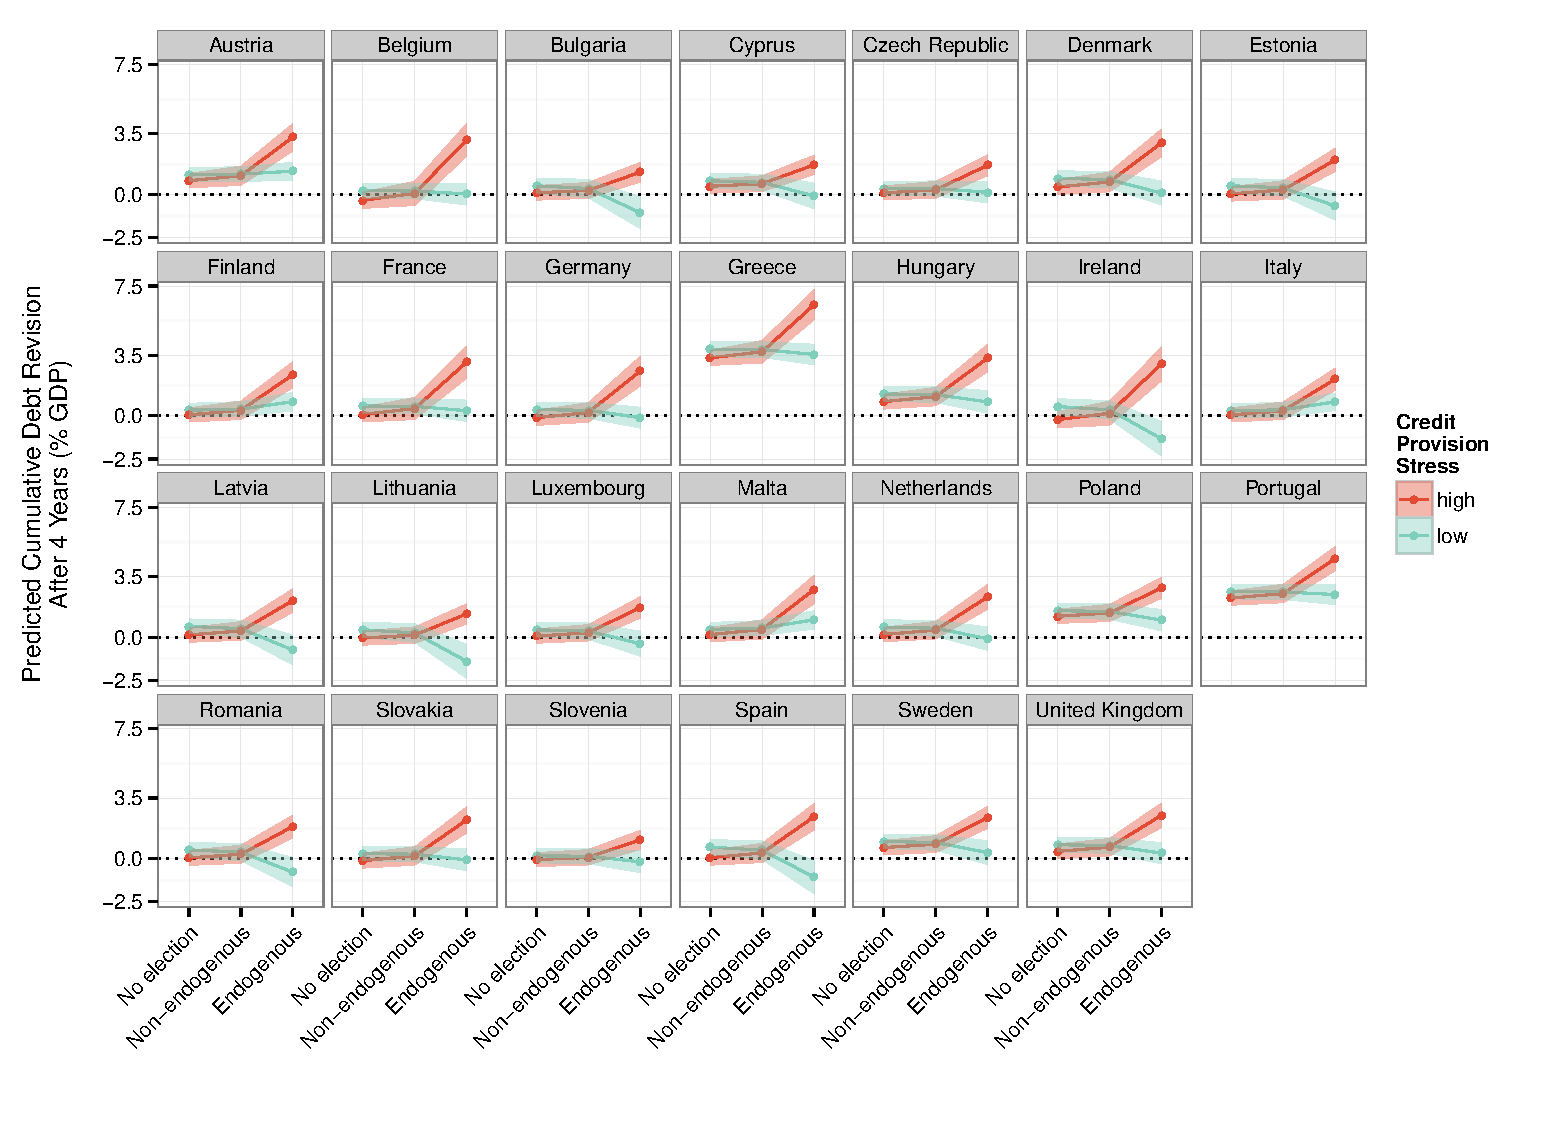
\includegraphics[scale=0.7]{figures/country_predict_required.pdf}
    \end{center}

	{\scriptsize{High and Low stress values refer to country minimum and maximum FinStress scores in the sample.\\
    Croatia excluded due to a small number of revision years.\\
    Shaded areas show 95\% confidence intervals.
}}

\end{figure}

\begin{figure}
    \caption{Marginal Effect of a Non-Endogenous Election at Various Levels of Financial Market Stress on \textbf{Deficit} Revisions}
    \label{me_finstress_non_endog_deficit}
    \begin{center}
        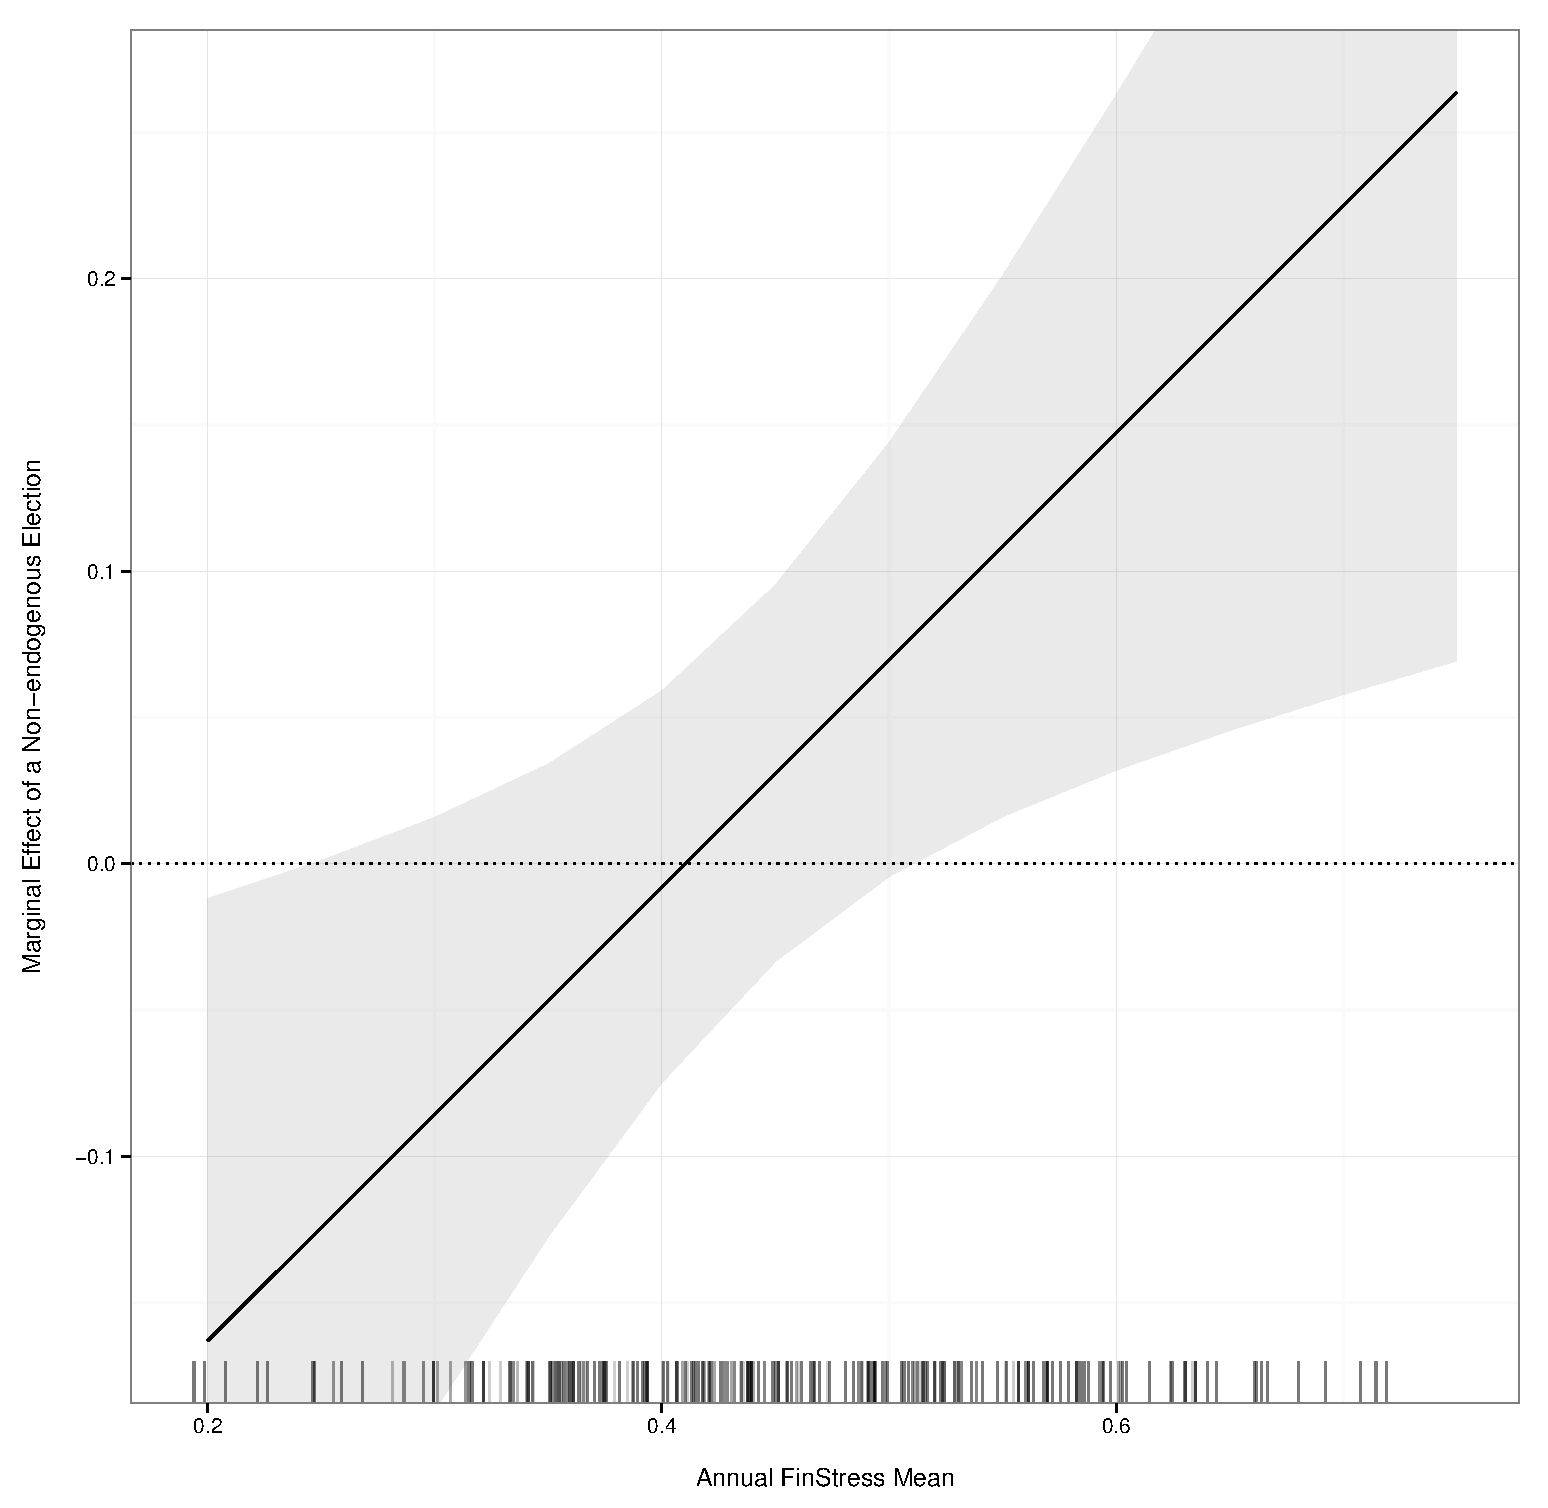
\includegraphics[scale=0.4]{figures/finstress_non_endog_deficit_me.pdf}
    \end{center}

	{\scriptsize{Shaded area represents 95\% confidence interval.}}

\end{figure}


\section{Conclusion}

In this paper we have attempted to understand government fiscal rule stretching behavior during financial market stress and crises. The European Union provides a unique opportunity for studying this behavior as it has an independent monitor that frequently revisits and revises member state balance sheet statistics. We significantly deepen findings in previous work that elections are associated with revisions to government debt and deficit figures. We specifically examine behavior during endogenous elections and periods of financial market stress. We find that government debt rule stretching is is much more prevalent during financial crises and when elections are endogenous.

Overall, it appears that deficit rule stretching, at least during our sample, may more about avoiding running afoul of the Stability and Growth Pact's three percent deficit limit rather than a result of electoral incentives or financial market stress. Nonetheless, more work is needed to understand the relationships between non-endogenous elections and rule stretching that we observe here.

A major takeaway from our work is that even among a group of developed economies with generally strong economic institutions, that fiscal rule stretching is common and can significantly affect our knowledge about government spending and financial obligations. This is especially true during financial market stress. As such independent government accounting agencies, such as Eurostat, are a crucial component of get the numbers right, even if it takes a few years.


\clearpage

\bibliographystyle{apsr}
\bibliography{main.bib}

\clearpage

\section*{Appendix}

We ran a number of tests to examine whether or not governments select into endogenous elections according to the prevailing level of financial market stress. Table \ref{finstress_endog} shows results from a logistic regression where we tried to predict having an endogenous election in a year for our sample based on annual average FinStress level. We can see that there is a null result. We made a similar finding when running a multinomial logistic regression (not shown), with endogenous and non-endogenous elections as categories and no election as the reference category.


% Table created by stargazer v.5.2 by Marek Hlavac, Harvard University. E-mail: hlavac at fas.harvard.edu
% Date and time: Thu, Dec 03, 2015 - 13:27:54
\begin{table}[!htbp] \centering 
  \caption{Logistic Regression Estimation of Having an Endogenous Election} 
  \label{finstress_endog} 
\begin{tabular}{@{\extracolsep{5pt}}lc} 
\\[-1.8ex]\hline 
\hline \\[-1.8ex] 
 & \multicolumn{1}{c}{\textit{Dependent variable:}} \\ 
\cline{2-2} 
\\[-1.8ex] & Endogenous Election \\ 
\hline \\[-1.8ex] 
 FinStress & $-$0.137 \\ 
  & (0.154) \\ 
  & \\ 
 Constant & 0.195$^{*}$ \\ 
  & (0.111) \\ 
  & \\ 
\hline \\[-1.8ex] 
Country FE? & Yes \\ 
Observations & 216 \\ 
Log Likelihood & 31.788 \\ 
Akaike Inf. Crit. & $-$7.575 \\ 
\hline 
\hline \\[-1.8ex] 
\textit{Note:}  & \multicolumn{1}{r}{$^{*}$p$<$0.1; $^{**}$p$<$0.05; $^{***}$p$<$0.01} \\ 
\end{tabular} 
\end{table} 


\end{document}
